\chapter{Gegenüberstellung}
\thispagestyle{fancy}
\section{Planung}

Das Thema Planung wird unter folgenden fünf Aspekten betrachtet:
\begin{enumerate}
\item Release-Planung
\item Priorisierung
\item Planungssicherheit
\item Planungsaufwands
\item Nachvollziehbarkeit
\end{enumerate}

\subsection{Release-Planung}

{\Large Scrum:} \cite{planningReleaseScrum} \medskip

Der Release-Plan ist ein höhergestellter Plan, der mehrere Sprints beinhaltet und während der Release-Planung festgelegt wird. Der Plan definiert welche Features umgesetzt werden und wann diese erfüllt sind. Er dient auch dazu den Fortschritt innerhalb des Projekts verfolgen zu können. Es können mehrere Releases während des Projekts geplant werden oder einfach ein finales Release am Ende des Projekts. \medskip

Um eine Release-Planung durchführen zu können, muss Folgendes bekannt sein:
\begin{itemize}
\item Ein priorisiertes Scrum-Backlog
\item Die Ressourcen des Scrum-Teams
\item Zielerfüllungsbedingungen
\end{itemize}
Ein Release-Plan kann Termin- oder Feature-geführt sein.\smallskip

Bei Termin-geführten Projekten wird spezifiziert, welche Features bis zu einem bestimmten Termin erfüllt werden können.\smallskip
Kommt es bei einem Termin-geführten Projekt zu Verzögerungen, so muss gegebenenfalls der Termin angepasst werden. Dies muss in Abstimmung mit dem Kunden gemacht werden.

Bei Feature-geführten Projekten wird spezifiziert, bis zu welchem Termin das Feature erfüllt ist. Kommt es bei Feature-geführten Projekten zu Verzögerungen, so muss zusammen mit dem Kunden besprochen werden, welche Features gegebenenfalls weggelassen werden können oder entsprechend angepasst werden müssen.\smallskip

Wie der Backlog ist auch der Release-Plan bei Scrum nicht statisch. Dieser kann sich mit dem Backlog ändern oder auch nach jedem Sprint wieder diskutiert und überarbeitet werden.
\bigskip 

{\Large DAD:} \cite{planningReleaseDad} \medskip

In DAD wird die Release Planung initial in der Inception Phase gemacht. Der Leitfaden empfiehlt für die Releaseplanung folgende sechs Fragen zu beantworten.
\begin{itemize}
	\item Wer wird an der Planung beteiligt sein?
	\item Was ist der Umfang unseres Planungsaufwands?
	\item Was ist unsere Gesamtstrategie, die diesen Plan vorantreibt?
    \item Wie detailliert sollte unser Plan sein?
    \item Welche Kadenzen wird das Team annehmen?
    \item Welchen Ansatz zur Schätzung werden wir wählen?
\end{itemize}
Damit soll sichergestellt werden, dass grundlegende Managementfragen gegenüber den Stakeholdern beantwortet sind. Zudem wird erreicht, dass eine durchführbare Strategie besteht und zwischen Stakeholder und Delivery Team ein gemeinsames Verständnis existiert.


\subsection{Priorisierung}

{\Large Scrum:} \cite{planningPrioScrum} \medskip

Das Scrum-Team priorisiert zusammen mit dem Product-Owner die Tasks/Stories aus dem Scrum-Backlog. Wichtig dabei ist, dass nicht nur priorisiert, sondern auch sortiert werden muss. Beim Sortieren wird auch die Reihenfolge von Abläufen berücksichtigt. Die Priorisierung geht mit der Sortierung Hand in Hand. \smallskip

Weiter achtet Scrum auch darauf, dass die wertvollsten Inkremente frühstmöglich umgesetzt werden.\bigskip 

{\Large DAD:} \cite{planningPrioDad} \medskip

Die Priorisierung bei DAD verhält sich ähnlich wie die Release-Planung. Grundsätzlich gilt das Rolling-Wave-Modell. Dass heisst, dass höher priorisierte Features detaillierter spezifiziert werden und tief priorisierte nur grob. Die Priorisierung kann jederzeit wieder angepasst werden.


\subsection{Planungsumfang}

{\Large Scrum:} \medskip

In Scrum betrifft der Umfang immer direkt das Produkt. Der Scope beinhaltet Features ausgedrückt z.B. als User Stories. Diese sind im Scrum-Backlog abgelegt und verwaltet.
\bigskip 

{\Large DAD:} \cite{planningScopeDad} \medskip

DAD geht hier einen Schritt weiter und definiert nicht nur Features sondern sogenannte Working-Items. Bei denen werden auch nicht-funktionale Anforderungen definiert wie z.B. Schulungen, Ferien, Unterstützung anderer Teams usw.	


\subsection{Planungsaufwand}

{\Large Scrum:} \medskip

Der Planungsaufwand von Scrum ist relativ gering und ist im iterierenden Prozess von Scrum bereits integriert. Die Planung wird bei Scrum vor jedem Sprint im sogenannten Sprint Planning gemacht. Dabei werden die zu erledigenden Items definiert. Schlussendlich wird der Umfang des Sprints vom ganzen Team bestätigt.\bigskip 

{\Large DAD:} \medskip

Initial ist der Planungsaufwand bei DAD hoch. Man muss nebst der eigentlichen Planung des Produkts auch diverse Analysen von Ist-Zuständen bezüglich Ressourcen und Zuständen innerhalb des Unternehmens machen um die Rahmenbedingungen für das Projekt zu legen. Während der Construction Phase ist der Planungsaufwand analog demjenigen von Scrum.


\subsection{Risikomanagement}

{\Large Scrum:} \medskip

Bei Scrum wird das Risikomanagement hauptsächlich durch die Kommunikation zwischen dem Kunden und Team geführt. Diese geht über den Product Owner. Dabei muss der Kunde durch seinen stetigen Einfluss mögliche Risiken ausschliessen können. Er kann dies mittels Akzeptanzkriterien beeinflussen.\newline
Aus Team-interner Sicht ist die Definition of Done das Kontrollinstrument, um Qualität aber auch Vollständigkeit sicherzustellen.
Als weiteres Instrument dient die Review am Ende jedes Sprints. An jener werden dem Kunden die umgesetzten Items präsentiert und er kann Einfluss nehmen, sowie Missverständnisse aufdecken und klären.

\bigskip 

{\Large DAD:} \medskip

Um das Risiko von Fehlkommunikation zu verringern werden bei DAD gegenüber Scrum leichte Meilensteine eingeführt, bei denen ein Abgleich mit dem Kunden stattfindet. \medskip

Weiter sieht DAD die Planung von festen Releases vor. Damit soll regelmässig Software zur Verfügung gestellt werden, um ein Feedback des Kunden zu erhalten und frühzeitig festzustellen, ob man die Anforderungen so erfüllen kann. Dies ist gleich wie bei Scrum.

\section{Zusammenarbeit}


\subsection{Koordination im Team}

{\Large Scrum:} \cite{planningReleaseScrum} \medskip

Scrum geht grundsätzlich von einer selbstorganisierten Koordination aus. Einzig der Scrum Master hat eine "koordinierende" Rolle, jedoch nur im Bezug auf den Prozess und Schnittstellen ausserhalb des Projekts.
Als wichtigstes Instrument für Koordination in Scrum oder auch allgemein in agilen Vorgehensmodellen dient die Kommunikation mit den anderen Team-Mitgliedern. Dies wird in Scrum mit regelmässigen Treffen/Aussprachen realisiert. Wie zum Beispiel das Daily Stand-up oder Scrum of Scrums (Team übergreifend), welche speziell für die Koordination angedacht sind. Weitere Routinen wie Daily Scrum oder die Reflektion dienen auch der Koordination und deren Verbesserung, auch wenn das nicht primär ihr Ziel ist.
\bigskip 

{\Large DAD:} \cite{planningReleaseDad} \medskip

DAD möchte, dass folgende Fragen bezüglich Koordination in einem Scrum-Team geklärt sind, um eine effektive Organisation innerhalb des Teams zu haben.
\begin{itemize}
	\item 	Wie werden Informationen innerhalb des Teams ausgetauscht?
	\item 	Wer darf die vom Team erstellten Artefakte aktualisieren? 
	\item 	Wie werden wir uns innerhalb des Teams koordinieren?
	\item 	Wenn wir Teil eines größeren Teams sind, wie werden wir dann innerhalb dieses Teams koordinieren?
	\item 	Wie werden wir mit Enterprise-/IT-Teams wie Enterprise Architects und Data Managern zusammenarbeiten?
	\item 	Wie werden wir unsere Release-/Einsatzplanung mit dem Rest des Unternehmens koordinieren?
	\item 	Wenn wir geografisch verteilte Teammitglieder haben, wie werden wir dann mit ihnen zusammenarbeiten?
\end{itemize}
Innerhalb des Teams soll also klar definiert sein, mit welchen Routinen (tägliches Treffen, Video-Konferenzen, usw.) Informationen zwischen den Teammitgliedern ausgetauscht werden und welche Tools dazu verwendet werden. Auch soll die Zuständigkeit geregelt sein wer die finalen Artefakten verwaltet, dass es hier keine Überschneidungen oder Unklarheiten gibt.
\medskip

Weiter muss gerade bei agilen Teams innerhalb eines Unternehmen auch die Koordination mit anderen Teams/Abteilungen geregelt sein.
\medskip

Was oft vernachlässigt wird, ist die Koordination mit Teammitglieder an anderen geografischen Orten. Der Informationsaustausch wird hier anspruchsvoller, da direkte verbale Kommunikation, welche die effektivste ist, nicht möglich ist.


\subsection{Rolle und Aufgaben des Kunden}

{\Large Scrum:} \cite{planningPrioScrum} \medskip

Der Kunde soll in Scrum während des ganzen Projektes immer involviert sein. Folgende Möglichkeiten gibt es den Kunden zu involvieren:
\begin{itemize}
	\item Der Kunde wird zum im Initial-Meeting mit eingeladen.
	\item Backlog wird zusammen mit dem Kunden verwaltet.
	\item Der Kunde nimmt auch an Reviews teil, um Arbeiten zu besprechen und als abgeschlossen zu definieren.
\end{itemize}
Durch den konsequenten Miteinbezug des Kunden wird das Risiko vermindert, dass der Kunde nicht zufrieden ist, da er fortlaufend Einfluss nehmen kann und mit seiner Teilnahme auch frühe Schritte/Arbeiten bestätigt.
\bigskip 

{\Large DAD:} \cite{planningPrioDad} \medskip

DAD hat bezüglich dem Kunden eine andere auch radikalere Haltung. In DAD will man den Begriff "Kunde" nicht verwenden, sondern nur Stakeholder. Dieser werden in folgende Gruppen unterteilt:
\begin{itemize}
	\item Endbenutzer: Personen die das Produkt schlussendlich verwenden.
	\item Vorstehende: Personen die schlussendlich entscheiden, welches Produkt beschafft wird, Bezahlungen freigeben werden, usw.
	\item Partner: Unterhalter, Betreiber, Entwickler von externen Systemen, Juristen, usw.
	\item Interne: Personen innerhalb des Entwicklungsteams und welche technische oder geschäftliche Dienste liefern
\end{itemize}
Für ein Produkt gibt es nur Stakeholders und es gilt dessen Anforderung genau zu ermitteln und festzulegen. Dazu werden für alle Stakeholder die Bedürfnisse gleichwertig ermittelt und miteinbezogen. \smallskip

Man will also bewusst ein Produkt, dass alle Stakeholder gleich berücksichtigt und nicht nur den "bezahlenden Kunden" hauptsächlich priorisieren. Denn nur so wird der "abbezahlende Kunde" auch ein nachhaltiges und erfolgreiches Produkt erhalten können.
\medskip
Als wichtig wird auch herausgehoben, dass das Projekt im "wir"-Kontext betrachtet wird und nicht im "ihr". Es gibt nicht den Kunden und das Entwicklungsteam, sondern das Projekt betrifft alle gleich.


\section{Zuständigkeit}
\subsection{Rollen}
{\Large Scrum:} \medskip

In Scrum gibt es drei Rollen. Den Scrum Master, den Product Owner und die Team Member. 
\begin{figure}[H]
	\centering
	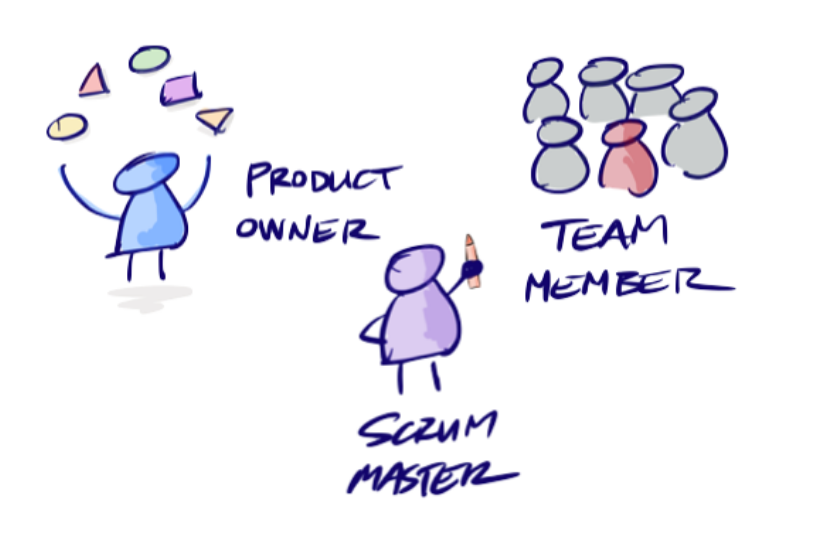
\includegraphics[scale=0.8]{scrum_roles}
	\caption{Scrum Rollen}
	\label{fig:scrumrollen}
\end{figure}

Der \textbf{Product Owner} ist die Ansprechperson für Kunden und Stakeholder. Er nimmt die Anforderungen entgegen, priorisiert diese und gibt diese an das Team weiter. Der Product Owner kann aber auch direkt der Kunde sein. In beiden Fällen vertritt er aber die fachliche Sicht, beurteilt die Qualität, Usability und Performance. \medskip

Der \textbf{Scrum Master} dient dem Scrum Team um die gewünschte Performance zu erreichen. Er ist verantwortlich, dass der Prozess zielgerichtet ausgeführt werden kann. Er nimmt sich Problemen, sogenannten Impediments, an und löst diese - mit oder ohne Team. Der Scrum Master fördert den Fortschritt des Teams und lenkt dieses, falls der Fortschritt nicht wie geplant vorankommt. Zudem organisiert die Scrum Zeremonien - Retrospektive, Review-Meeting, Daily Standups - und sorgt für den Informationsfluss zwischen Team und Product Owner. Er ist sozusagen die gute Seele des Teams. \medskip

Das \textbf{Scrum Team}, oder kurz Team, ist das zentrale Element im Scrum Prozess. Es setzt die Anforderungen um. In Scurm besteht ein Team aus fünf bis zehn Personen. Grössere Teams sollten in mehrere unabhängige Teams aufgetrennt werden. Sehr wichtig bei Scrum ist, dass das Team selbst organisiert. Es bestimmt schlussendlich selbst, welche Anforderungen es im Sprint umsetzten will. Dabei beachtet es, dass es am Ende jedes Sprints ein «Increment of  Potentially Shippable Functionality» liefert. In einem Scrum Team sind immer die Disziplinen vorhanden, welche es für das Erreichen des Ziels benötigt.
\bigskip 

{\Large DAD:} \medskip

Im Gegensatz zu Scrum werden in DAD zusätzliche Rollen definiert. In DAD werden einzelne Zuständigkeiten explizit aufgeführt, welche in Scrum im Team vereint werden. DAD verwendet gewisse Rollen aus dem Agilen Manifest (Team Member und Product Owner), aber unterscheidet hierbei primäre und unterstützende Rollen. Zu den primären Rollen zählen Team Lead, Product Owner, Team Member, Architecture Owner und Stakeholder. Zu den unterstützenden Rollen zählen Spezialisten, Independent Tester, Domänen-Experten, Technische Experten und Integratoren.
\begin{figure}[H]
	\centering
	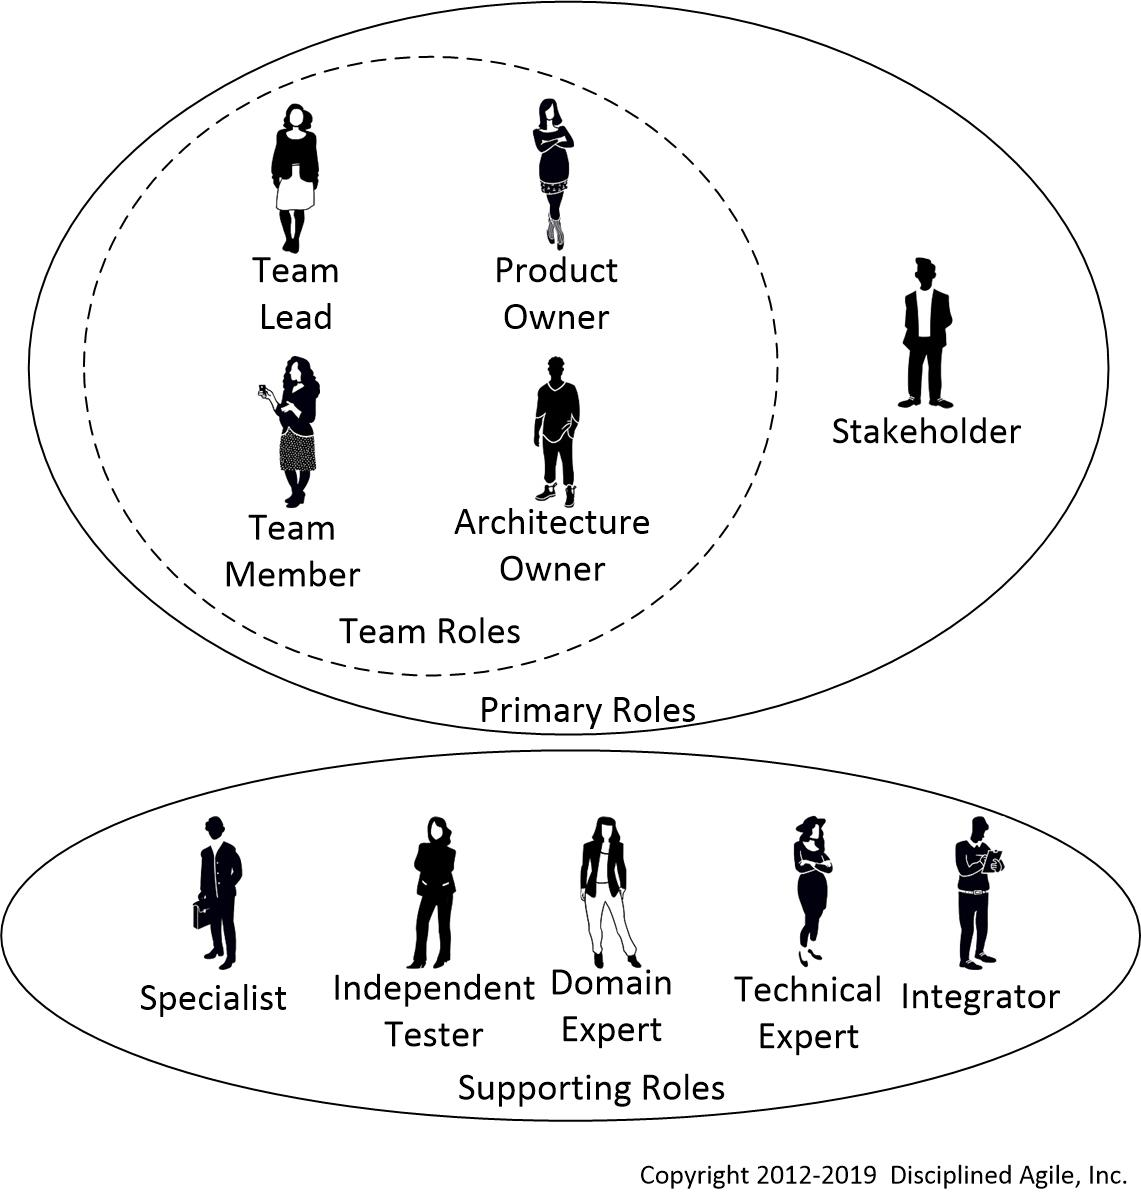
\includegraphics[scale=0.8]{DAD-Roles}
	\caption{DAD Rollen}
	\label{fig:dadrollen}
\end{figure}

DAD wurde somit stark auf die Bedürfnisse von Unternehmen weiterentwickelt, um Bedürfnisse aus den bestehenden Firmenstrukturen mit Prozessen, Programmen und Rollen anzuwenden. DAD unterstützt mit den sehr spezifischen Rollen hierarchische Unternehmensstrukturen.
\bigskip 


In diesem Punkt unterscheiden sich die zwei Methoden wesentlich. Warum hat Scrum drei Rollen, DAD hingegen zehn? Scrum konzentriert sich hauptsächlich auf Führungs- und Change-Management-Aspekte während der Konstruktion und hat daher Rollen, die dies widerspiegeln. DAD hingegen konzentriert sich explizit auf den gesamten Delivery Lifecycle und alle Aspekte der Lösungsbereitstellung, einschließlich der technischen Aspekte, die Scrum auslässt. Mit einem größeren Umfang kommen also mehr Rollen hinzu. Weil DAD beispielsweise Fragen der agilen Architektur umfasst, beinhaltet es auch eine Rolle des Architecture Owners. Scrum adressiert keine Architektur und beinhaltet auch keine solche Rolle.

\subsection{Verantwortlichkeiten}

In diesem Aspekt wird beschrieben wie die Verantwortlichkeiten auf die Rollen verteilt sind und welche Verantwortlichkeiten im Prozess wahrgenommen werden müssen.

{\Large Scrum:} \medskip

In Scrum hat jede Rolle ihre Verantwortlichkeit im Prozess. Der Scrum Master hat in erster Linie die Verantwortung zur Einhaltung des Prozesses und der Scrum Spielregeln. Wie bereits im Kapitel Rollen beschrieben hat er die Verantwortung zur Beseitigung von Hindernissen.

Der Product Owner hat die Verantwortung die Vision und Wünsche des Kunden an das Team weiterzugeben. Er ist die Stimme der Stakeholder und somit verantwortlich die Bedürfnisse des Kunden zu identifizieren.

Die grösste Verantwortung wird jedoch dem Team zugeteilt. Es legt den Umfang fest, welchen es umsetzt - das sogenannte Sprint Goal. Es verpflichtet sich dazu das Sprint Goal umzusetzen. Bei Problemen oder Störungen muss das Team zeitnah mit dem Kunden bzw. mit dem Product Owner in Kontakt treten, um gegebenenfalls das Sprint Goal anzupassen. Da das Team selbstorganisiert ist, liegt es in seiner Verantwortung, wie das Ziel erreicht wird.

\smallskip
{\Large DAD:} \medskip

Da es in DAD mehr Rollen als in Scrum gibt, sind auch die Verantwortlichkeiten expliziter.
Wir gehen hier nur auf die Verantwortlichkeiten der primären Rollen ein.

Der Team Lead hat in DAD eine ähnliche Funktion und Verantwortlichkeiten wie der Scrum Master. Er dient dem Team als Coach. Er schaut, dass das Team performant arbeiten kann und fördert das Team in der Verbesserung ihrer Arbeitsweise.

Der Product Owner in DAD unterscheidet sich kaum vom PO in Scrum. Auch in DAD ist er die Stimme des Kunden. Er priorisiert die Aufgaben und versucht die Fragen des Teams zu beantworten oder leitet diese an den Kunden weiter.

Der Architecture Owner ist verantwortlich für die Umsetzung der architektonischen Entscheide. Er trifft die Architektur Entscheide, erstellt das Design der Gesamtlösung und übernimmt die Weiterentwicklung davon. Oft ist der Architecture Owner auch der Lead Entwickler. Manchmal wird er auch Softwarearchitekt oder Solutionarchitekt genannt. Der AO ist keine hierarchische Rolle. Er arbeitet mit dem Team und trifft die Entscheidungen in Absprache mit ihm.

Wie in Scrum hat auch das Team in DAD die grösste Verantwortung. Darunter zählen:

\begin{itemize}
	\item Eine Lösung zu finden, die den Bedürfnissen der Stakeholder entspricht.
	\item Optimierte Nutzung der Ressourcen
	\item Bereitschaft zu einer umfassenden Zusammenarbeit innerhalb Ihres Teams, auch ausserhalb Ihres Fachgebiets.
	\item Informationsaustausch über alle Arbeiten, die im Gange sind.
	\item Andere in Ihren Fähigkeiten und Erfahrungen zu coachen.
	\item Erweiterung Ihrer Kenntnisse und Fähigkeiten ausserhalb Ihres Fachgebiets.
	\item Teilnahme an den Meetings.
	\item Proaktiv nach Wegen zur Verbesserung der Teamleistung suchen
	\item Vermeiden, dass Arbeiten außerhalb der aktuellen Iteration ohne Zustimmung des Teams angenommen werden.
	\item Arbeit so früh wie möglich validieren und mit anderen zusammenzuarbeiten
\end{itemize}

Diese Punkte sind ziemlich Deckungsgleich wie jene die im agilen Manifest geschildert werden. 

\subsection{Zielerfüllung}

\medskip
{\Large Scrum:} \medskip

Jedes Artefakt, welches in einer Iteration (Sprint) umgesetzt wird, wird durch Akzeptanzkriterien beschrieben. Diese werden zusammen mit oder durch den Kunden definiert. Anhand dieser Akzeptanzkriterien wird ein Artefakt gemessen. Die Akzeptanzkriterien dienen dem Team, nebst einer genauen Beschreibung des Artefakts, zur Erreichung des Sprint Ziels.

In Scrum wird nach jedem Sprint die sogenannte Review gemacht. Hier wird dem Kunden das Produkt bzw. die umgesetzten Artefakte präsentiert. Hier hat der Kunde die Möglichkeit lenkend einzugreifen. Da in Scrum in kurzen Iterationen gearbeitet wird, kann der Kunde schnell und zeitnah Einfluss auf Missverständnisse nehmen.

Das Team definiert zudem die Definition of Done. Die DoD definiert, wann ein Task abgeschlossen ist. Diese Kriterien müssen nicht zwingend deckend zu den Akzeptanzkriterien sein. Oft hat die DoD umfassendere Punkte wie bspw. Tests, Dokumentation, Review etc.

\medskip
{\Large DAD:} \medskip

Grundsätzlich hat DAD dieselben Mechanismen zur Sicherstellung der Zielerreichung wie Scrum. Nach jeder Iteration wird, wie in Scrum auch, die Iteration zusammengefasst. Den Stakeholdern wird eine Demo der umgesetzten Tasks gezeigt und es wird entschieden ob man mit dem Vorgehen weitermacht. Zum Abschluss wird eine Analyse über den Way of Work gemacht und die nötigen Verbesserungen werden angebracht.

In DAD wird zudem eine gemeinsame Vision mit den Stakeholdern erstellt. Dies ist ein weiteres Mittel zu Sicherstellung der Zielerreichung.

In DAD besteht jede Phase, Inception, Construction, Transition, aus mehreren Goals. Ein Goal kann einmal oder mehrmals durchlaufen werden. Ein Goal besteht aus einem oder mehreren Decision Points.

\begin{figure}[H]
	\centering
	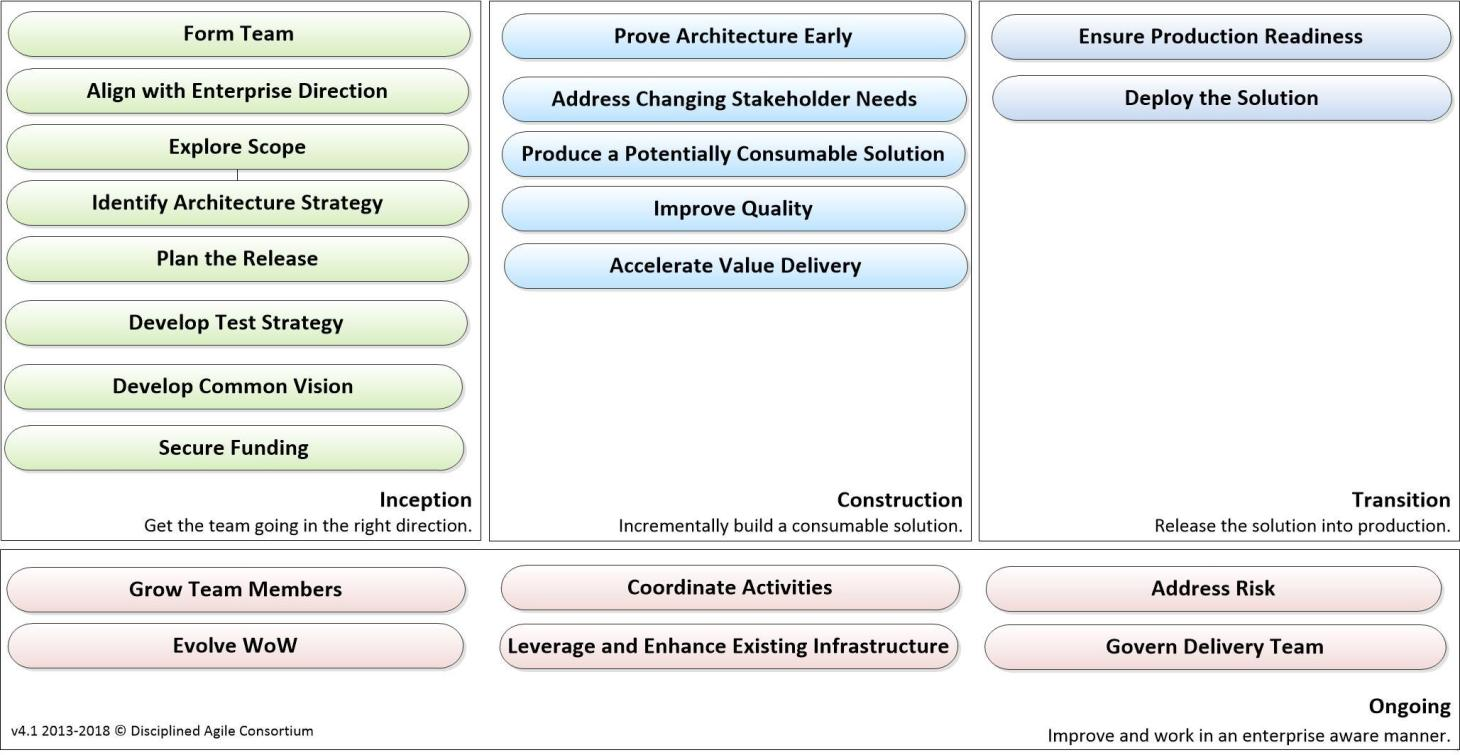
\includegraphics[width=\textwidth]{Lifecycle-Goals.jpg}
	\caption{Lifecycle Goals}
	\label{fig:goals}
\end{figure}

Die Decision Points und Goals dienen der Sicherstellung des Prozesses und somit auch der Erreichung der Ziele.

\subsection{Rollenkonflikte}

In Scrum wie auch in DAD sind die Teams selbstorganisiert, was impliziert, dass Hierarchien in Frage gestellt werden. Gerade in Scrum werden explizite Disziplinen nicht gesucht. Scrum fordert, dass alle Mitglieder eines Teams möglichst jede Aufgabe im Sprint abarbeiten können. Ein exklusiver Tester, Programmierer oder Architekt passt somit nicht optimal in ein Scrum Team. Ein gutes Team kann dies aber berücksichtigen und die Nachteile kompensieren. Dies sollte aber wenn möglich in erfahrenen Teams gemacht werden.

DAD bietet hier Unterstützung indem zusätzliche Rollen explizit adressiert werden. So ist nicht nur der Architecture Owner explizit aufgeführt, sondern DAD weist auch unterstützende, sogenannte Supporting Roles, auf. Diese können je nach Bedürfnis des Teams und des Projekts verwendet werden. So kann bei Bedarf ein Tester oder ein Domänen Experte hinzugezogen werden. DAD versucht hier die Rollenkonflikte zu mindern. Jedoch ist darauf hinzuweisen, dass auch DAD Hierarchien in Frage stellt und somit selbstorganisierte Teams fördert.



\section{Empfehlung}


IN PROGRESS

Grundsätzlich wäre der Ansatz mit DAD sicher spannend. Ihr Team kann nach wie vor mit Scrum arbeiten und Sie haben die Möglichkeit mit den erwähnten Instrumenten wie leichte Meilensteine, Release Planung der agilen Entwicklung Einfluss zu nehmen und dem ganzen einen ein Rahmen zu geben. \newline
Jedoch wird Sie das Einführen dieses Vorgehensmodell hohen Aufwand kosten. Vor allem muss für das saubere Anwenden von DAD viel Analyse von bestehenden Prozessen und Zuständen innerhalb Ihres Unternehmens betrieben werden.
Im Bereich der Releaseplanung bietet DAD den Vorteil, dass die Release Planung bereits frühzeitig im Projekt definiert wird. Gegenüber Scrum werden hier viel tiefergehende Fragen geklärt um das Projekt im Einklang mit der unternehmerischen Strategie zu bringen. Dabei wird früh mit den beteiligten Stakeholdern ein gemeinsames Verständnis gefunden, nach welchem das weitere Vorgehen definiert ist. \newline
Die Priorisierung von Scrum und DAD verhält sich sehr ähnlich. Bei beiden wird iterativ eine Priorisierung der Inkremente vorgenommen, wobei die wichtigsten Features jeweils den Vortritt erhalten. DaD geht zusätzlich nach dem Rolling-Wave-Modell vor und spezifiziert höher priorisierte Features detaillierter als tiefer priorisierte. Wird dieser Vorgang angewendet, so geschieht im Projekt Team dadurch eine Fokussierung aufs Wesentliche. Das Wichtige wird genauer besprochen, während die Details bei, zu diesem Zeitpunkt noch weniger wichtigen Anforderungen, zeitsparend weggelassen werden können. \newline
Der Planungsausfwand ist bei DAD initial sicher höher, dafür bringt dieser im Planungsumfang einige Vorteile. So werden z.B. auch nicht funktionale Anforderungen definiert, welche über das eigentliche Projekt hinaus gehen. Somit ist DAD im Vergleich zu Scrum besser mit bestehenden Unternehmensstrukturen und spezifischen Anforderungen der Unternehmen ans Projekt vereinbar. \newline
Scrum definiert für die Zusammenarbeit verschiedene Rollen innerhalb des Projekt Teams. Das Modell klärt aber keine oder nur wenige Fragen bezüglicher der Koordination mit der Unternehmung und den darin bereits vorhandenen Rollen. Hier bietet DAD einen grossen Vorteil, da es genau auf diese Fragen eingeht. Somit können mit DAD weiterführende Fragen zur Integration des Projekt Teams in die Unternehmung geklärt werden und somit das Modell optimal im bestehenden Unternehmen integriert werden. So werden im DAD Modell auch einzelne Rollen, die im Scrum in den Aufgabenbereich des Teams fallen, explizit aufgeführt. Diese sind spezifisch auf die Bedürfnisse von bestehenden Firmenstrukturen ausgelegt. Insbesondere ist DAD auf hierarchische Unternehmensstrukturen ausgelegt, welche durch die definierten Rollen im Modell übernommen werden können.\newline
Gegenüber dem Kunden gibt es grosse Unterschiede zwischen Scrum und DAD. Scrum priorisiert den zahlenden Kunden, während DAD versucht alle Stakeholder gleichwertig mit einzubeziehen. Daraus ergibt sich mit DAD eine umfassendere Rückmeldung zu den einzelnen Releases. Das führt zwar zu einem komplexeren Gesamtbild, dafür können Stakeholder Bedürfnisse früh herauskristallisiert und entsprechend früh in den Entwicklungsprozess miteinbezogen werden. Wird dies dem Kunden gegenüber entsprechend kommuniziert, können dadurch grosse Vorteile, sowie Kosteneinsparungen im Projekt erreicht werden. \newline
Zusammenfassend kann festgehalten werden, dass Scrum und DAD sich zwar sehr ähnlich sind, DAD aber einige wichtige Vorteile für Ihr Unternehmen bietet. Neben den vielfältigeren Rollen, welche so ausgelegt sind, dass sie in die bestehenden Unternehmensstrukturen eingebettet werden können, werden mit DAD auch Unternehmensstrategische Ziele berücksichtigt. Dies sind wichtige Fragen, die für die beiden bestehenden Unternehmen geklärt werden müssen und genau dafür ist DAD ausgelegt. Ein weiterer Vorteil für die Einführung eines neuen Modells, in diesem Falle DAD, wäre die Tatsache dass sich beide Unternehmen auf neue Strukturen einlassen müssten, was im gegebenen Fall sicher von Vorteil ist. Zwar ist der Planungsaufwand höher als bei einer Übernahme eines bereits im Aufwand stehenden Modells, doch die gemeinsame Bewältigung der Aufgabe wird auch ein gemeinsames Verständnis zwischen den beiden Unternehmen fördern und die Teams vereinen. Aus diesen genannten Gründen empfehlen wir das Modell DAD in ihrem Unternehmen einzuführen.





	